\documentclass{report}
\usepackage[utf8]{inputenc}
\usepackage[T1]{fontenc}
\usepackage{graphicx}
\usepackage{listings}
\usepackage{url}
\usepackage[utf8]{inputenc}
\usepackage[spanish]{babel}
\lstloadlanguages{[ANSI]C}
\usepackage{color}
\usepackage{fullpage}

\lstset{
language=[ANSI]C,               % the language of the code
basicstyle=\footnotesize,       % the size of the fonts that are used for the code
numbers=left,                   % where to put the line-numbers
numberstyle=\footnotesize,      % the size of the fonts that are used for the line-numbers
stepnumber=1,                   % the step between two line-numbers. If it's 1, each line will be numbered
numbersep=5pt,                  % how far the line-numbers are from the code
backgroundcolor=\color{white},  % choose the background color. You must add \usepackage{color}
showspaces=false,               % show spaces adding particular underscores
showstringspaces=false,         % underline spaces within strings
showtabs=false,                 % show tabs within strings adding particular underscores
frame=single,                   % adds a frame around the code
tabsize=2,                      % sets default tabsize to 2 spaces
captionpos=t,                   % sets the caption-position to bottom
breaklines=true,                % sets automatic line breaking
breakatwhitespace=false,        % sets if automatic breaks should only happen at whitespace
title=\lstname,                 % show the filename of files included with \lstinputlisting; also try caption instead of title
%escapeinside={\%*}{*)},        % if you want to add a comment within your code
%morekeywords={*,...}           % if you want to add more keywords to the set
}


\begin{document}
\title{\textit{Kernel} para la arquitectura \textit{IA32}}
\author{Endika Gutierrez Salas, Jon Ander Peñalba y David Gómez Hernández}
\maketitle

\tableofcontents

\chapter{Introducción}

El objetivo de este trabajo es crear un \textit{kernel} para la arquitectura \textit{IA32} que cargaremos en una máquina virtual.
Para arrancar el kernel necesitaremos además un gestor de arranque, para lo que utilizaremos \textit{GRUB}\footnote{\textit{GRUB} - \url{http://www.gnu.org/software/grub/}}.

La mayor parte del kernel está escrita en \textit{C}, pero hay partes que es necesario hacer en ensamblador.
Una de estas partes es el código de arranque, que está en el fichero \textit{arch/loader.s}.
Este código lleva a cabo algunas operaciones necesarias para poder cargar el \textit{kernel} y después llama a nuestra función principal (\textit{kernel\_main}).

\lstinputlisting[language={[x86masm]Assembler}]{../arch/loader.s}

\chapter{La Pantalla}

Una vez tenemos un \textit{kernel} que puede ejecutarse hay que usar algún periférico de salida para mostrar lo que está haciendo.
Como este \textit{kernel} es muy básico, usamos el periférico de salida más sencillo, la pantalla en modo texto.

\section{La Teoría}

El \textit{kernel} se inicia con \textit{GRUB} en modo texto.
Esto quiere decir que tiene disponible un \textit{framebuffer} (área de memoria) que controla una pantalla de caracteres de 80 de ancho por 25 de alto.
Este será el modo en que el \textit{kernel} operará.

El \textit{framebuffer} es accesible como \textit{RAM} normal, en la dirección \textit{0xB8000}.
Pero es importante dejar claro que a pesar de esto no es \textit{RAM} normal, es parte de la memoria de vídeo dedicada del controlador
\textit{VGA} a la que se le ha realizado un mapeo de memoria vía hardware al espacio lineal de direcciones. Es una diferencia importante.
El \textit{framebuffer} es un array de palabras de 16 \textit{bits}, cada valor de 16 \textit{bits} representando un carácter.

En \textit{ASCII} (no se soporta el \textit{Unicode} en modo texto) solo se usan 8 \textit{bits} para representar el carácter,
así que disponemos de 8 \textit{bits} extra que el controlador \textit{VGA} usa para designar los colores del texto y del fondo (4 \textit{bits} cada uno).
La división de este valor de 16 \textit{bits} queda entonces como se muestra en la figura \ref{fig:vga_word}.

\begin{figure}[htb]
\centering
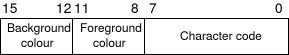
\includegraphics[scale=0.7]{word_format.png}
\caption{Elemento del array de vídeo}
\label{fig:vga_word}
\end{figure}

El controlador \textit{VGA} tiene también algunos puertos en el \textit{bus} principal de \textit{E/S}, que se puede usar para enviar instrucciones específicas.
Los más importantes para nosotros son el registro de control en \textit{0x3D4} y el registro de datos en \textit{0x3D5},
mediante los cuales podemos actualizar la posición del cursor.

\section{La Práctica}
\subsection{Código de la pantalla}

A continuación se muestra la cabecera del código de pantalla.

\lstinputlisting{../arch/screen.h}

Como se puede ver es muy sencillo, solo define dos funciones (una para escribir un carácter y la otra para borrar la pantalla) y unas \textit{macros} para definir los colores.

Internamente este código hace solamente lo más básico.
Imprime los caracteres uno a uno y va actualizando la posición del cursor teniendo en cuenta que algunos caracteres especiales como el salto de línea necesitan un trato especial.

\begin{lstlisting}[title=Función que escribe un carácter en pantalla]
// Write a char at the cursor's current position
void arch_putc_color(uint8_t c, uint8_t color)
{
    switch (c) {
        case '\n':
            while (cursor_pos % SCREEN_CHARS_WIDE)
                video_buffer[cursor_pos++] = (color << 8) | ' ';
            break;
        case '\r':
            do {
                video_buffer[cursor_pos] = (color << 8) | ' ';
            } while (--cursor_pos % SCREEN_CHARS_WIDE);
            break;
        case '\b':
            if (cursor_pos)
                video_buffer[cursor_pos--] = (color << 8) | ' ';
            break;
        case '\t':
            do {
                video_buffer[cursor_pos++] = (color << 8) | ' ';
            } while (cursor_pos % TAB_SIZE);
            break;
        default:
            video_buffer[cursor_pos++] = (color << 8) | c;
            break;
    }

    if (cursor_pos >= SCREEN_SIZE)
        scroll();

    update_cursor();
}
\end{lstlisting}

Para borrar la pantalla simplemente recorre todo el \textit{buffer} de vídeo, lo llena de espacios y posteriormente pone el cursor en la primera posición.
Y si al escribir un carácter llega al final del \textit{buffer}, recorre todas las lineas desde la segunda copiándolas a la línea anterior y luego borra la ultima línea.

\begin{lstlisting}[title=Función que hace \textit{scroll}]
INLINE void scroll(void)
{
    // Move all lines one row up
    int i = SCREEN_CHARS_WIDE;
    for (; i < SCREEN_SIZE; ++i)
        video_buffer[i-SCREEN_CHARS_WIDE] = video_buffer[i];

    // Erase the last line
    for (i -= SCREEN_CHARS_WIDE; i < SCREEN_SIZE; ++i)
        video_buffer[i] = SCREEN_COLOR(BLACK, L_GREY) << 8 | ' ';

    cursor_pos -= SCREEN_CHARS_WIDE;
}
\end{lstlisting}

\subsection{\textit{kprintf}}

De momento el código es suficiente para escribir por pantalla, pero lo realmente útil es disponer de algo parecido al \textit{printf} de \textit{C}.
Así que hemos definido nuestro propio \textit{printf} para el \textit{kernel}.

\lstinputlisting{../lib/kprintf.h}

Este código lo que hace es primero extraer todos los parámetros que se le han pasado a la función y después mostrarlos en el formato deseado.

\begin{lstlisting}[title=Función que imprime una cadena de caracteres]
void vkprintf(const char* format, va_list vl)
{
    uint8_t color = SCREEN_COLOR(BLACK, L_GREY);

    for (const char *s = format; *s; s++) {
        if (*s == '%') {
            s++;

            switch (*s) {
                case 'c': { // Character
                    char c = va_arg(vl, char);
                    arch_putc_color(c, color);
                    break;
                }
                case 's': { // String
                    const char* str = va_arg(vl, const char*);
                    for (; *str; ++str)
                        arch_putc_color(*str, color);
                    break;
                }
                case 'd': // Signed decimal integer
                case 'i': {
                    int d = va_arg(vl, int);
                    kprint_int(d, 10, false, color);
                    break;
                }
                case 'u': { // Unsigned decimal integer
                    unsigned int d = va_arg(vl, unsigned int);
                    kprint_int(d, 10, true, color);
                    break;
                }
                case 'o': { // Unsigned octal
                    int d = va_arg(vl, int);
                    kprint_int(d, 8, false, color);
                    break;
                }
                case 'x': { // Unsigned hexadecimal integer
                    int d = va_arg(vl, int);
                    kprint_int(d, 16, false, color);
                    break;
                }
                case 'X': { // Unsigned hexadecimal integer (capital letters)
                    int d = va_arg(vl, int);
                    kprint_int(d, 16, true, color);
                    break;
                }
                case '$': // Change color
                    color = va_arg(vl, char);
                    break;
                case '%': // %
                    arch_putc_color('%', color);
                    break;
                default: // Do nothing
                    break;

            }

        } else {
            arch_putc_color(*s, color);
        }
    }
}
\end{lstlisting}
% '$

\chapter{La \textit{GDT} y la \textit{IDT}}

La \textit{GDT} y la \textit{IDT} son tablas de descriptores.
Son matrices (\textit{arrays}) de \textit{flags} y \textit{bits} que describen la operación del sistema
de segmentación (en el caso de la \textit{GDT}), o la tabla del vector de interrupciones (\textit{IDT}).

\section{Tabla Global de Descriptores (teoría)}

La arquitectura x86 tiene dos métodos de protección de memoria y de dar memoria virtual - segmentación y paginación.

Con segmentación, cada acceso a memoria es evaluado respecto a un segmento. Esto quiere decir que a la dirección base del segmento se le suma la dirección de memoria y después se comprueba con la longitud del segmento. Se puede pensar en el segmento como una ventana al espacio de direcciones - El proceso no sabe si es una ventana, todo lo que ve es un espacio lineal de direcciones que empieza en cero y llega hasta la longitud del segmento.

Con paginación, el espacio de direcciones en bloques (normalmente de 4KB, pero esto puede cambiar), llamados páginas. Cada página puede ser mapeada en la memoria física - mapeada en lo que se llama 'frame'. O puede ser no-mapeada. De este modo se pueden crear espacios de memoria virtual.

Cada uno de estos métodos tienen sus ventajas, pero la paginación es mucho mejor. La segmentación se está volviendo obsoleta a gran velocidad como método de protección de memoria y memoria virtual, aunque sigue utilizándose. De hecho, la arquitectura x86-64 requiere memoria plana (un segmento con una base de 0 y un límite de 0xFFFFFFFF) para que algunas de sus instrucciones operen de un modo correcto.

Sin embargo, la paginación está totalmente incorporada a la arquitectura x86. Es imposible evitarla. Aquí vamos a explicar como crear la Tabla Global de Descriptores - una lista de descriptores de segmento.

Como se ha mencionado antes, vamos a intentar y crear un modelo de memoria plano. La ventana del segmento debería comenzar en 0x0000000 y etenderse hasta 0xFFFFFFFF (el final de la memoria). Sin embargo, hay una cosa que la segmentación puede hacer y la paginación no puede: establecer el nivel de privilegio.

El nivel de privilegio es 0 siendo éste el más privilegiado y 3 el menos. Los procesos en el nivel cero se dice que se ejecutan en modo-kernel o modo-supervisor, porque pueden usar instrucciones como \textit{sti} y \textit{cli}, algo que muchos procesos no pueden. Normalmente, los niveles 1 y 2 están sin usar. Técnicamente pueden acceder a un mayor subconjunto de instrucciones del modo-supervisor que el nivel 3. Algunas arquitecturas de microkernel usan estos para ejecutar procesos servidor o controladores.

Un descriptor de segmento lleva en su interior un número que representa el nivel al que si aplica. Para cambiar el nivel de privilegio (que haremos más adelante), entre otras cosas, necesitamos segmentos que representen tanto al nivel 0 como al nivel 3.

\section{Tabla Global de Descriptores (práctica)}

GRUB puede crear una GDT por ti, el problema es que no sabes donde está esa GDT o lo que hay en ella. De modo que puedes sobrescribirla accidentalmente, tras lo cual el ordenador fallaría y se reiniciaría.

En el x86 tenemos 6 registros de segmentación. Cada uno tiene una compensación para la GDT. Hay sc (segmento de código), sd (segmento de datos), se (segmento extra), sf, sg, ss (segmento de pila). El segmento de código debe referenciar a un descriptor que esté puedo como 'segmento de código'. Existe un flag para esto en el byte de acceso. El resto deben referenciar a un descriptor que esté puesto como 'segmento de datos'.

\begin{figure}[htb]
\centering
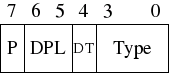
\includegraphics[scale=0.5]{gdt_idt_gdt_format_2.png}
\end{figure}

\subsubsection{descriptor\_tables.h}

Una entrada de GDT tiene esta pinta:

\begin{lstlisting}
// This structure contains the value of one GDT entry.
// We use the attribute 'packed' to tell GCC not to change
// any of the alignment in the structure.
struct gdt_entry_struct
{
   u16int limit_low;           // The lower 16 bits of the limit.
   u16int base_low;            // The lower 16 bits of the base.
   u8int  base_middle;         // The next 8 bits of the base.
   u8int  access;              // Access flags, determine what ring this segment can be used in.
   u8int  granularity;
   u8int  base_high;           // The last 8 bits of the base.
} __attribute__((packed));
typedef struct gdt_entry_struct gdt_entry_t;
\end{lstlisting}

Muchos de los campos se explican por sí mismos. El formato del byte de acceso se da arriba y aquí damos el formato del byte de granularidad.

\begin{figure}[htb]
\centering
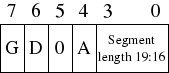
\includegraphics[scale=0.5]{gdt_idt_gdt_format_1.png}
\end{figure}

\textbf{P} Está el segmento presente (1 = si)

\textbf{DPL} Nivel de privilegio del descriptor

\textbf{DT} Tipo de descriptor

\textbf{Type} Tipo de segmento - segmento de código / segmento de datos

\textbf{G} Granularidad (0 = 1 byte, 1 = 1kbyte)

\textbf{D} Tamaño

\textbf{0} Siempre debería ser cero.

\textbf{A} Disponible para el uso del sistema )(siempre cero).

Para decir al procesador dónde encontrar nuestra GDT, hay que darle la dirección de una estructura especial de puntero.

\begin{lstlisting}
struct gdt_ptr_struct
{
   u16int limit;               // The upper 16 bits of all selector limits.
   u32int base;                // The address of the first gdt_entry_t struct.
}
 __attribute__((packed));
typedef struct gdt_ptr_struct gdt_ptr_t;
\end{lstlisting}

La base es la dirección de la primera entrada en nuestra GDT, el límite es el tamaño de la table menos uno (la última dirección válida de la tabla).

Esas definiciones de struct deberían estar en un archivo de cabecera, descriptor\_tables.h, junto a un prototipo.

\begin{lstlisting}
// Initialisation function is publicly accessible.
void init_descriptor_tables();
\end{lstlisting}

\subsubsection{descriptor\_tables.c}

En descriptor\_tables.c tenemos unas cuantas declaraciones:

\begin{lstlisting}
//
// descriptor_tables.c - Initialises the GDT and IDT, and defines the 
// default ISR and IRQ handler.
// Based on code from Bran's kernel development tutorials.
// Rewritten for JamesM's kernel development tutorials.
//

#include "common.h"
#include "descriptor_tables.h"

// Lets us access our ASM functions from our C code.
extern void gdt_flush(u32int);

// Internal function prototypes.
static void init_gdt();
static void gdt_set_gate(s32int,u32int,u32int,u8int,u8int);

gdt_entry_t gdt_entries[5];
gdt_ptr_t   gdt_ptr;
idt_entry_t idt_entries[256];
idt_ptr_t   idt_ptr;
\end{lstlisting}

Hay que fijarse en la función gdt\_flush - será definida en un archivo ASM y cargará el puntero de nuestra GDT por nosotros.

\begin{lstlisting}
// Initialisation routine - zeroes all the interrupt service routines,
// initialises the GDT and IDT.
void init_descriptor_tables()
{
   // Initialise the global descriptor table.
   init_gdt();
}

static void init_gdt()
{
   gdt_ptr.limit = (sizeof(gdt_entry_t) * 5) - 1;
   gdt_ptr.base  = (u32int)&gdt_entries;

   gdt_set_gate(0, 0, 0, 0, 0);                // Null segment
   gdt_set_gate(1, 0, 0xFFFFFFFF, 0x9A, 0xCF); // Code segment
   gdt_set_gate(2, 0, 0xFFFFFFFF, 0x92, 0xCF); // Data segment
   gdt_set_gate(3, 0, 0xFFFFFFFF, 0xFA, 0xCF); // User mode code segment
   gdt_set_gate(4, 0, 0xFFFFFFFF, 0xF2, 0xCF); // User mode data segment

   gdt_flush((u32int)&gdt_ptr);
}

// Set the value of one GDT entry.
static void gdt_set_gate(s32int num, u32int base, u32int limit, u8int access, u8int gran)
{
   gdt_entries[num].base_low    = (base & 0xFFFF);
   gdt_entries[num].base_middle = (base >> 16) & 0xFF;
   gdt_entries[num].base_high   = (base >> 24) & 0xFF;

   gdt_entries[num].limit_low   = (limit & 0xFFFF);
   gdt_entries[num].granularity = (limit >> 16) & 0x0F;

   gdt_entries[num].granularity |= gran & 0xF0;
   gdt_entries[num].access      = access;
}
\end{lstlisting}

Analicemos ese código un poco. init\_gdt inicializa la estructura del puntero gdt - el límite es el tamaño de cada entrada gdt multiplicado por 5 (tenemos 5 entradas) ¿Por qué 5? Tenemos un segmento de código y uno de datos para el kernel, segmento de código y de datos para modo usuario y una entrada null. Esto debe estar presente o ocurrirán cosas malas.

gdt\_init prepara 5 descriptores llamando gdt\_set\_gate. gdt\_set\_gate mueve y cambia los bits, y debería explicarse por sí misma echándole un buen vistazo. Hay que fijarse en que la única cosas que cambia entre los 4 descriptores de segmento es el byte de acceso - 0x9A, 0x92, 0xFA, 0xF2. Se puede ver, si se mapean los bits y se comparan con el diagrama de arriba que los bits que cambian son los campos de tipo y DPL. DPL es el nivel de privilegio del descriptor - 3 para código de usuario y 0 para código de kernel. El tipo especifica si el segmento es un segmento de código o de datos (el procesador comprueba esto a menudo, y puede ser la fuente de mucha frustración).

Finalmente tenemos nuestra función ASM que escribirá el puntero GDT.

\begin{lstlisting}
[GLOBAL gdt_flush]    ; Allows the C code to call gdt_flush().

gdt_flush:
   mov eax, [esp+4]  ; Get the pointer to the GDT, passed as a parameter.
   lgdt [eax]        ; Load the new GDT pointer

   mov ax, 0x10      ; 0x10 is the offset in the GDT to our data segment
   mov ds, ax        ; Load all data segment selectors
   mov es, ax
   mov fs, ax
   mov gs, ax
   mov ss, ax
   jmp 0x08:.flush   ; 0x08 is the offset to our code segment: Far jump!
.flush:
   ret
\end{lstlisting}

Esta funcion toma el primer parametro pasado (in esp+4), carga el valor al que apunta a la GDT (usando la instrucción lgdt), carga entonces los selectores de segmento para segmentos de código y datos. Hay que fijarse en que cada entrada de la GDT es de 8 bytes y que el descriptor de código del kernel es el segundo segmento, así que su compensación es 0x08. De esta forma el descriptor de datos del kernel es el tercero, así que su compensación es 16 = 0x10. Aquí se mueve el valor 0x10 a los registros del segmento de datos ds, es, fd, gs, ss. Para cambiar el segmento de código es ligeramente diferente; debemos hacer un salto hacía delante. Esto cambia la impicidad del segmento de código.

\section{Tabla de Descriptores de Interrupción (teoría)}

Hay veces en se quiere interrumpir al procesador. Se quiere detener lo que está haciendo, y forzarlo a hacer algo diferente. Un ejemplo de esto es cuando un se dispara una petición de interrupción (IRQ) de reloj o de teclado. Una interrupción es como una señal de POSIX - te dice que algo de interés ha ocurrido. El procesador puede registrar 'signal handlers' (handlers de interrupción) que pueden ocuparse de la interrupción y volver después al semento de código que se estaba ejecutando antes de que se disparase. Las interrupciones pueden ser disparadas externamente, por medio de IRQ, o internamente, por medio de la instrucción 'int n'. Hay razones muy útiles para querer disparar interrupciones por software, pero eso será para otro capítulo.

La \textit{Tabla de Descriptores de Interrupción} dice al procesador donde encontrar handlers para cada interrupción. Es muy parecida a la GDT. Es un array de entradas, cada una de las cuales corresponde a un número de interrupción. Hay 256 posibles número de interrupción, de modo que 256 han de ser definidos. Si se da una interrupción y no hay una entrada para ella (incluso una entrada a NULL sería correcta), el procesador se reiniciaría.

\subsection{Fallos, traps y excepciones}

El proecesaro necesitara a veces mandar una señal al kernel. Algo muy importante habrá ocurrido, como una división entre cero, o un fallo de página. Para hacer esto usa las 32 primeras interrupciones. Es por tanto doblemente importante que todas éstas estén mapeadas y no sean nulas - de lo contrario la CPU fallaría y se reiniciaría (bochs entraría en pánico con un error 'unhandled exception').

Las interrupciones especiales dedicadas a la CPU se muestran a continuación.

\begin{itemize}
	\item 0 - Excepción de división entre cero
	\item 1 - Excepción de depuración
	\item 2 - Interrupción no mascarable
	\item 3 - Excepción de breakpoint
	\item 4 - 'Into detected overflow'
	\item 5 - Excepción fuera de límites
	\item 6 - Excepción de código de operación invalido
	\item 7 - Excepción no coprecesador
	\item 8 - Doble fallo, da un código de error
	\item 9 - Invasión  de coprocesador
	\item 10 - Mala TSS (genera un código de error)
	\item 11 - Segmento no presente (genera un código de error)
	\item 12 - Fallo de pila (genera un código de error)
	\item 13 - Fallo de protección general (genera un código de error)
	\item 14 - Fallo de página (genera un código de error)
	\item 15 - Excepción de interrupción desconocida
	\item 16 - Fallo de coprocesador
	\item 17 - Excepción de comprobación de alineado
	\item 18 - Machine check exception
	\item 19-31 - Reservador
	
\end{itemize}

\section{Tabla de Descriptores de Interrupción (práctica)}

\subsection{descriptor\_tables.h}

Debemos añadir mas definiciones a  descriptor\_tables.h:

\begin{lstlisting}
// A struct describing an interrupt gate.
struct idt_entry_struct
{
   u16int base_lo;             // The lower 16 bits of the address to jump to when this interrupt fires.
   u16int sel;                 // Kernel segment selector.
   u8int  always0;             // This must always be zero.
   u8int  flags;               // More flags. See documentation.
   u16int base_hi;             // The upper 16 bits of the address to jump to.
} __attribute__((packed));
typedef struct idt_entry_struct idt_entry_t;

// A struct describing a pointer to an array of interrupt handlers.
// This is in a format suitable for giving to 'lidt'.
struct idt_ptr_struct
{
   u16int limit;
   u32int base;                // The address of the first element in our idt_entry_t array.
} __attribute__((packed));
typedef struct idt_ptr_struct idt_ptr_t;

// These extern directives let us access the addresses of our ASM ISR handlers.
extern void isr0 ();
...
extern void isr31();
\end{lstlisting}

El formato del byte Flags es muy similar a la entrada GDT y los structs ptr. El formato del flag se muestra a continuación. Los 5 bits más bajos deben ser constantes a 0b0110, 14 en decimal. DPL especifica el nivel de privilegio del que esperamos ser llamados, en este caso 0, pero según vayamos avanzando necesitaremos cambiarlo a 3. El bit P indica si la entrada está presente. Cualquier descriptor con este bit a cero causará una excepción "Interrupción no Manekada".

\subsection{descriptor\_tables.c}

\begin{lstlisting}

We need to modify this file to add our new code.

...
extern void idt_flush(u32int);
...
static void init_idt();
static void idt_set_gate(u8int,u32int,u16int,u8int);
...
idt_entry_t idt_entries[256];
idt_ptr_t   idt_ptr;
...
void init_descriptor_tables()
{
  init_gdt();
  init_idt();
}
...
static void init_idt()
{
   idt_ptr.limit = sizeof(idt_entry_t) * 256 -1;
   idt_ptr.base  = (u32int)&idt_entries;

   memset(&idt_entries, 0, sizeof(idt_entry_t)*256);

   idt_set_gate( 0, (u32int)isr0 , 0x08, 0x8E);
   idt_set_gate( 1, (u32int)isr1 , 0x08, 0x8E);
   ...
   idt_set_gate(31, (u32int)isr32, 0x08, 0x8E);

   idt_flush((u32int)&idt_ptr);
}

static void idt_set_gate(u8int num, u32int base, u16int sel, u8int flags)
{
   idt_entries[num].base_lo = base & 0xFFFF;
   idt_entries[num].base_hi = (base >> 16) & 0xFFFF;

   idt_entries[num].sel     = sel;
   idt_entries[num].always0 = 0;
   // We must uncomment the OR below when we get to using user-mode.
   // It sets the interrupt gate's privilege level to 3.
   idt_entries[num].flags   = flags /* | 0x60 */;
}
\end{lstlisting}

Se añade también esto a gdt.st:

\begin{lstlisting}

[GLOBAL idt_flush]    ; Allows the C code to call idt_flush().

idt_flush:
   mov eax, [esp+4]  ; Get the pointer to the IDT, passed as a parameter. 
   lidt [eax]        ; Load the IDT pointer.
   ret
   
\end{lstlisting}


\subsection{interrupt.s}

Tenemos el código que indicará a la CPU dónde encontrará el código para gestionar las interrupciones, sin embargo aun no hay nada escrito.

Cuando el procesador recibe una interrupción, guarda el contenido de los registros esenciales (puntero de instruccion, puntero de pila, segmentos de código y datos, registro flags) en la pila. Después encuentra la localización del gestor de interrupción de nuestra IDT y salta a él.

Ahora, justamente como con los gestores de señales de POSIX, no se da ninguna información acerca de que interrupción se invoca cuando se ejecuta el gestor. Así que, por desgracia, no podemos tener un gestor común, debemos escribir un gestor diferente para cada una de las interrupciones que queremos gestionar. Esto es bastante pobre, ya que queremos mantener la cantidad de código duplicado al mínimo. Se puede hacer esto escribiendo gestores que simplemente hagan un push del numero de interrupción (hardcodeado en ASM) a la pila y llamar a un una función de gestión común.

Eso es insignificante, pero desafortunadamente tenemos otro problema: algunas interrupciones hacen un push de un código de error a la pila. No se puede llamar a la función común sin un marco común de pila, así que para esas que no hacen push de código de error hacemos un push de uno falso, para que la pila sea la misma.

\begin{lstlisting}

[GLOBAL isr0]
isr0:
  cli                 ; Disable interrupts
  push byte 0         ; Push a dummy error code (if ISR0 doesn't push it's own error code)
  push byte 0         ; Push the interrupt number (0)
  jmp isr_common_stub ; Go to our common handler.
  
\end{lstlisting}

Esta rutina funcionaría, pero 32 versiones de ella parecen un monton de código de modo que se puede usar el macro de NASM para acortar esto.

\begin{lstlisting}
%macro ISR_NOERRCODE 1  ; define a macro, taking one parameter
  [GLOBAL isr%1]        ; %1 accesses the first parameter.
  isr%1:
    cli
    push byte 0
    push byte %1
    jmp isr_common_stub
%endmacro

%macro ISR_ERRCODE 1
  [GLOBAL isr%1]
  isr%1:
    cli
    push byte %1
    jmp isr_common_stub
%endmacro
\end{lstlisting}

Se puede hacer una función gestora de stubs de la siguiente manera

\begin{lstlisting}


ISR_NOERRCODE 0
ISR_NOERRCODE 1
...

\end{lstlisting}


Un vistazo rápido al manual de intel hará que nos demos cuenta de que solo las interrupciones 8, 10-14 incluyen un push de código de rror a la pila. El resto requiere un push de un código falso.


Hay que crear una función de gestión común en ensamblador y también crear una función de gestión común de más alto nivel, en C.

\begin{lstlisting}
; In isr.c
[EXTERN isr_handler]

; This is our common ISR stub. It saves the processor state, sets
; up for kernel mode segments, calls the C-level fault handler,
; and finally restores the stack frame.
isr_common_stub:
   pusha                    ; Pushes edi,esi,ebp,esp,ebx,edx,ecx,eax

   mov ax, ds               ; Lower 16-bits of eax = ds.
   push eax                 ; save the data segment descriptor

   mov ax, 0x10  ; load the kernel data segment descriptor
   mov ds, ax
   mov es, ax
   mov fs, ax
   mov gs, ax

   call isr_handler

   pop eax        ; reload the original data segment descriptor
   mov ds, ax
   mov es, ax
   mov fs, ax
   mov gs, ax

   popa                     ; Pops edi,esi,ebp...
   add esp, 8     ; Cleans up the pushed error code and pushed ISR number
   sti
   iret           ; pops 5 things at once: CS, EIP, EFLAGS, SS, and ESP
   
\end{lstlisting}


Este segmento de código es el gestor de interrupción común. Usa en primer lugar el comando 'pusha' para hacer un push todos los registros de propósito general a la pila. Usa el comando 'popa' para restaurarlos al final. También coge el selector de segmento actual y hace un push a la pila, prepara todos los registros de segmento para el selector de datos del kernel, y los restaura después. Esto no tendrá un efecto inmediato, pero cuando cambiemos a modo usuario si que lo tendrá. Hay que fijarse en que también invoca un gestor de interrupción de un nivel más alto: el isr\_handler.

Cuando se lanza una interrupción, el procesador automáticamente hace push de la información sobre el estado del procesador a la pila. Se hace push del segmento de código, puntero de instrucción, registro flags, segmento de pila y puntero de pila. La instrucción IRET está específicamente diseñada para volver de una interrupción. Hace pop de estos valores de la pila y devuelve al procesador al estado que estaba inicialmente.

\subsection{isr.c}

\begin{lstlisting}
//
// isr.c -- High level interrupt service routines and interrupt request handlers.
// Part of this code is modified from Bran's kernel development tutorials.
// Rewritten for JamesM's kernel development tutorials.
//

#include "common.h"
#include "isr.h"
#include "monitor.h"

// This gets called from our ASM interrupt handler stub.
void isr_handler(registers_t regs)
{
   monitor_write("recieved interrupt: ");
   monitor_write_dec(regs.int_no);
   monitor_put('\n');
}

\end{lstlisting}

El gestor de interrupción imprime un mensaje en pantalla junto con el número de interrupción que se ha tratado. Usa una estructura registers\_t, que es una representación de todos los registros de los que hemos hecho push y está definido en isr.h:

\subsection{isr.h}


\begin{lstlisting}
//
// isr.h -- Interface and structures for high level interrupt service routines.
// Part of this code is modified from Bran's kernel development tutorials.
// Rewritten for JamesM's kernel development tutorials.
//

#include "common.h"

typedef struct registers
{
   u32int ds;                  // Data segment selector
   u32int edi, esi, ebp, esp, ebx, edx, ecx, eax; // Pushed by pusha.
   u32int int_no, err_code;    // Interrupt number and error code (if applicable)
   u32int eip, cs, eflags, useresp, ss; // Pushed by the processor automatically.
} registers_t;
\end{lstlisting}

\subsection{Prueba}


\begin{lstlisting}

asm volatile ("int $0x3");
asm volatile ("int $0x4");

\end{lstlisting}

\chapter{Paginación}

En este capítulo se explica como habilitar la paginación. La paginación tiene dos objetivos: protección de memoria y memoria virtual (ambos siendo intrínsecamente interdependientes)

\section{Memoria Virtual (teoría)}

Si se crea un programa como el siguiente en linux

\begin{lstlisting}
int main(char argc, char **argv)
{
  return 0;
}
\end{lstlisting}
, se compila y después se ejecuta 'objdump -f', se puede encontrar algo así.

\begin{lstlisting}
jamesmol@aubergine:~/test> objdump -f a.out

a.out:     file format elf32-i386
architecture: i386, flags 0x00000112:
EXEC_P, HAS_SYMS, D_PAGED
start address 0x080482a0
\end{lstlisting}

Hay que fijarse que la dirección de comienzo está en 0x80482a0, que está 128 MB en el interior del espacio de direcciones. Puede parecer extraño que este programa funcione perfectamente en máquinas con RAM inferior a 128MB.

Lo que realmente 've' el programa cuando lee y escribe en memoria es un espacio de dirección virtual. Partes del espacio virtual de direcciones están mapeadas a la memoria y partes no lo están. Si se intenta acceder a una parte no mapeada, el procesador el procesador genera un fallo de página, el sistema operativo lo captura y en sistemas POSIX genera una señal SIGSEV seguida de una SIGKILL.

Esta abstracción es extremadamente útil. Significa que los compiladores pueden producir un programa que confíe en que el código este en un lugar concreto de memoria siempre que se ejecute. Con memoria virtual, el proceso cree que, por ejemplo, está en 0x080482a0, sin embargo puede realmente estar en la la posición física de memoria 0x1000000. Y no solo eso, los procesos no pueden accidentalmente (o deliberadamente) dañar el código o datos de otros procesos.

Este tipo de memoria virtual es totalmente dependiente del soporte hardware. No puede ser emulado por software. Afortunadamente el x86 está provisto de esto. Se llama MMU (memory management unit) y se ocupa del mapeo de memoria debido a segmentación y paginación, formando una capa entre la CPU y la memoria (es de hecho parte de la CPU, pero eso es solo un detalle de implementación)


\section{Paginación como concreción de la memoria virtual}

La memoria virtual es un principio abstracto. Como tal requiere concreción a través de algun sistema o algoritmo. Tanto la segmentación como la paginación son métodos válidos para implementar la memoria virtual. Como se ha mencionado anteriormente, la segmentación se está quedando obsoleta. La paginación es la más nueva y mejor alternativa para la arquitectura x86.

La paginación trabaja dividiendo el espacio virtual de direcciones en bloques llamados páginas, que normalmente son de 4KB de tamaño. Las páginas pueden pueden ser mapeadas en frames, que son bloques del mismo tamaño en memoria física.


\subsection{Entradas de página}


Cada proceso tiene normalmente un conjunto diferente de mapeos de página, de modo que los espacios de memoria virtual sean independientes unos de otros. En la arquitectura x86 (32 bits), las páginas son fijas de un tamaño de 4KB. Cada página tiene su correspondiente palabra descriptor, que dice al procesador que que frame mapea. Hay que darse cuenta que ya que las páginas y los frames deben estar alineados a límites de 4KB (4KB siendo 0x1000 bytes), los 12 bits menos significativos de las palabras de 32 bits son siempre 0. La arquitectura se aprovecha de esto usándolos para almacenar información sobre la página, como si está presente, si está en modo kernel o en modo usuario, etc. La distribución está en el gráfico de la derecha.


\textbf{P}
    Activado si la página está presente en memoria

\textbf{R/W}
    Si está activado, la página se podrá escribir. Sino, la página será solamente de solo lectura. Esto no se aplica cuando se ejecuta código en modo kernel (a menos que se active un flag CR0)

\textbf{U/S}
    Si está activado, está es una página de modo usuario. Sino es una pagina de modo supervisor (modo kernel). El código en modo usuario no puede ni escribir ni leer páginas de modo kernel.

\textbf{Reserved}
    Estos se usan internamente por la CPU y no pueden ser manipulados.

\textbf{A}
    Activado si la página ha sido accedida (es activado por la CPU)

\textbf{D}
    Se activa si se ha escrito en la página (sucio)

\textbf{AVAIL}
    Estos 3 bits están sin utilizar y están disponibles para el uso del kernel.

\textbf{Dirección del frame de página}
    Los 20 bits altos del frame de dirección en memoria física.
    
\subsection{Directorios de páginas/tablas}


Para generar una tabla mapeando cada página de 4KB a un descriptor de 32 bits en un espacio de direcciones de 4GB se necesitan 4MB de memoria. Si se tienen 4GB de RAM físicos, no es mucho. Sin embargo, si se trabaja con una máquina que tiene 16MB de RAM, se pierde un cuarto de la memoria disponible. Lo que se quiere es algo progresivo, que ocupe una cantidad de espacio proporcional a la cantidad de RAM que se tiene.

No tenemos eso. Pero intel descubrió algo similar: un sistema de 2 nivel. Se informa a la CPU acerca de un directorio de páginas, que es una gran tabla de 4KB, de cuuyas entradas, cada una apunta a una tabla de página. La tabla de página es, de nuevo, de un tamaño de 4KB y sus entradas son entradas de páginas, descritas arriba.

De este modo, el espacio de direcciones de 4Gb puede ser enteramente cubierto con la ventaja de que si una tabla de página no tiene entradas, puede ser liberada y su bit de presencia desactivado en el directorio de páginas.

\subsection{Activando Paginación}

Activar la paginación es bastante sencillo.

Hay que copiar la localización del directorio de páginas en el registro CR3. Esto debe, por supuesto, ser una dirección física.
Activa el bit PG en el registro CR0. Esto se puede hacer mediante una OR con 0x80000000.


\section{Fallos de página}

Cuando un proceso proceso hace algo, al gestor de memoria "no le gusta", se lanza una interrupción por fallo de página. Estas son algunas situaciones que pueden hacer que esto ocurra:

Leer o escribir en un área de memoria que no este mapeada (entrada o tabla de página cuyo bit de presencia no esté activado)

El proceso esta en modo usuario e intenta escribir en una página de solo lectura.

El proceso está en modo usuario e intenta acceder a una página de solo modo kernel

la entrada de tabla de páginas esta corrupta, los bits reservados han sido sobreescritos.

La interrupción por fallo de página es la 14, y viendo lo puesto anteriormente se puede observar que esto lanza un código de error. Este código de eror da bastante información acerca de lo ocurrido.

\textbf{Bit 0}

	Si esta activado, el fallo no fue porque la página no estuviera presente. Si esta desctivado, la página no estaba presente.
    
    
\textbf{Bit 1}

	Si esta activado, la operación que causo el fallo fue de escritura, sino de lectura.
    
    
    
\textbf{Bit 2}

	Si está activado, el procesador se está ejecutando en modo usuario cuando ha sido interrumpido. Sino, se estaba ejecutando en modo kernel.
    
    
    
\textbf{Bit 3}

	Si está activado, el fallo ha sido causado por la sobreescritura de los bits de reserva.    
    
    
    
\textbf{Bit 4}

	Si esta activado, el fallo ocurre durante la instrucción fetch.
	
El procesador nos da también información: la dirección que causó el fallo. Está información está en el registro CR2. Cuidado ya que si el gestor de fallos de página causa el mismo otra excepción por fallo de página el registro se sobrescribirá, de modo que hay que salvarlo pronto.

\section{Aplicación practica}

A pesar de que casi se puede empezar a implementar hacen falta aun unas funciones de ayuda. Las más importantes de estas son las funciones de gestión de memoria. 


\subsection{Simple gestión de memoria con situación malloc}

Para gente con conocimientos de C++ el término 'placement new' puede resultar familiar. Esta es un versión de new que toma un parametro. En lugar de llamar a malloc, como normalmente haría, crea un objeto en la dirección especificada. Se usara un concepto muy similar.

Cuando el kernel está suficientemente iniciado, tendremos un kernel heap activo y operativo. El modo en que se codifica heaps normalmente requiere que la memoria virtual esté activada. De modo que se necesita una solución simple para asignar memoria antes de que el heap esté activo.

Segun se va asignando memoria, muy pronto en el inicialización del kernel, podemos asumir que nada que sea kmalloc() nunca necesitará ser kfree(). Esto simplifica las cosas mucho. Se puede tener un puntero (direccion de situación) a cierta memoria libre que enviamos al solicitado y despues incrementar, de modo:

\begin{lstlisting}

u32int kmalloc(u32int sz)
{
  u32int tmp = placement_address;
  placement_address += sz;
  return tmp;
}
\end{lstlisting}

Esto será suficiente. Sin embargo, existe otro requisito. Cuando asignemos tablas de páginas y directorios de páginas, deben de tener las páginas alineadas. Para poder hacer esto:

\begin{lstlisting}
u32int kmalloc(u32int sz, int align)
{
  if (align == 1 && (placement_address & 0xFFFFF000)) // If the address is not already page-aligned
  {
    // Align it.
    placement_address &= 0xFFFFF000;
    placement_address += 0x1000;
  }
  u32int tmp = placement_address;
  placement_address += sz;
  return tmp;
}
\end{lstlisting}

Desafortunadamente, hay otro requisito más. Se necesita conseguir la dirección física de la memoria asignada. 

\begin{lstlisting}
u32int kmalloc(u32int sz, int align, u32int *phys)
{
  if (align == 1 && (placement_address & 0xFFFFF000)) // If the address is not already page-aligned
  {
    // Align it.
    placement_address &= 0xFFFFF000;
    placement_address += 0x1000;
  }
  if (phys)
  {
    *phys = placement_address;
  }
  u32int tmp = placement_address;
  placement_address += sz;
  return tmp;
}
\end{lstlisting}



\begin{lstlisting}
u32int kmalloc_a(u32int sz);  // page aligned.
u32int kmalloc_p(u32int sz, u32int *phys); // returns a physical address.
u32int kmalloc_ap(u32int sz, u32int *phys); // page aligned and returns a physical address.
u32int kmalloc(u32int sz); // vanilla (normal).
\end{lstlisting}

Estas definiciones deberían estar en kheap.h/kheap.c.

\subsection{Difiniciones requeridas}

paging.h debería contener algunas definiciones de estructuras que facilitaran las cosas.

\begin{lstlisting}
#ifndef PAGING_H
#define PAGING_H

#include "common.h"
#include "isr.h"

typedef struct page
{
   u32int present    : 1;   // Page present in memory
   u32int rw         : 1;   // Read-only if clear, readwrite if set
   u32int user       : 1;   // Supervisor level only if clear
   u32int accessed   : 1;   // Has the page been accessed since last refresh?
   u32int dirty      : 1;   // Has the page been written to since last refresh?
   u32int unused     : 7;   // Amalgamation of unused and reserved bits
   u32int frame      : 20;  // Frame address (shifted right 12 bits)
} page_t;

typedef struct page_table
{
   page_t pages[1024];
} page_table_t;

typedef struct page_directory
{
   /**
      Array of pointers to pagetables.
   **/
   page_table_t *tables[1024];
   /**
      Array of pointers to the pagetables above, but gives their *physical*
      location, for loading into the CR3 register.
   **/
   u32int tablesPhysical[1024];
   /**
      The physical address of tablesPhysical. This comes into play
      when we get our kernel heap allocated and the directory
      may be in a different location in virtual memory.
   **/
   u32int physicalAddr;
} page_directory_t;

/**
  Sets up the environment, page directories etc and
  enables paging.
**/
void initialise_paging();

/**
  Causes the specified page directory to be loaded into the
  CR3 register.
**/
void switch_page_directory(page_directory_t *new);

/**
  Retrieves a pointer to the page required.
  If make == 1, if the page-table in which this page should
  reside isn't created, create it!
**/
page_t *get_page(u32int address, int make, page_directory_t *dir);

/**
  Handler for page faults.
**/
void page_fault(registers_t regs);
\end{lstlisting}

Fijarse en que los miembros tablesPhysical y physicalAddr de page\_table\_t.

El miembro physicalAddr es únicamente para cuando se clonan directorios de páginas. Recordar que en este punto, el nuevo directorio tendra una dirección de memoria virtual que no es la misma que la de memoria física. Se necesita la direccion física para decir a la CPU si se quiere cambiar de directorios.

El miembro tablesPhysical es similar. Es una solución a un problema: como accedes a tus tablas de páginas? Puede parecer sencillo, pero hay que recordar que un directorio de páginas debe contener direcciones físicas y no virtuales. Y la única manera de leer/escribir en memoria es usando direcciones virtuales.

Una solución a este problema es nunca acceder a la página de tablas directamente, sino mapear una table para apuntar hacia el directorio de páginas, de modo que accediendo a memoria en cierta dirección se podrán ver todas las tablas de páginas como si fuesen páginas, y todas las entradas de tabla de páginas como si fuesen integers normales.

El segundo método es para mantener 2 arrays para todo directorio de páginas. Uno con las direcciones físicas y de sus tablas de páginas (para dar a la CPU), y el otro conteniendo las direcciones viruales ( para así poder leer y escribir). Esto solamente genera un extra de 4KB por directorio de páginas, lo cual no es mucho.

\subsection{Asignación de frame}

Si se quiere mapear una página a un frame, necesitamos una manera de encontrar un frame libre. Por supuesto, se podría mantener un enorme array de 1s y 0s, pero esto sería un desperdicio enorme. No se necesitan 32 bits para solo contner 2 valores, esto se puede realizar con un bit. Asi que si se usa un bitset se usará 32 veces menos espacio.

Un bitset solo implementa tres funciones: set, test y clear. Se ha implementado una funcion para eficientemente encontrar el primer frame libre del bitmap.


\begin{lstlisting}

// A bitset of frames - used or free.
u32int *frames;
u32int nframes;

// Defined in kheap.c
extern u32int placement_address;

// Macros used in the bitset algorithms.
#define INDEX_FROM_BIT(a) (a/(8*4))
#define OFFSET_FROM_BIT(a) (a%(8*4))

// Static function to set a bit in the frames bitset
static void set_frame(u32int frame_addr)
{
   u32int frame = frame_addr/0x1000;
   u32int idx = INDEX_FROM_BIT(frame);
   u32int off = OFFSET_FROM_BIT(frame);
   frames[idx] |= (0x1 << off);
}

// Static function to clear a bit in the frames bitset
static void clear_frame(u32int frame_addr)
{
   u32int frame = frame_addr/0x1000;
   u32int idx = INDEX_FROM_BIT(frame);
   u32int off = OFFSET_FROM_BIT(frame);
   frames[idx] &= ~(0x1 << off);
}

// Static function to test if a bit is set.
static u32int test_frame(u32int frame_addr)
{
   u32int frame = frame_addr/0x1000;
   u32int idx = INDEX_FROM_BIT(frame);
   u32int off = OFFSET_FROM_BIT(frame);
   return (frames[idx] & (0x1 << off));
}

// Static function to find the first free frame.
static u32int first_frame()
{
   u32int i, j;
   for (i = 0; i < INDEX_FROM_BIT(nframes); i++)
   {
       if (frames[i] != 0xFFFFFFFF) // nothing free, exit early.
       {
           // at least one bit is free here.
           for (j = 0; j < 32; j++)
           {
               u32int toTest = 0x1 << j;
               if ( !(frames[i]&toTest) )
               {
                   return i*4*8+j;
               }
           }
       }
   }
}
\end{lstlisting}

Funciones para asginar y desasignar frames

\begin{lstlisting}
// Function to allocate a frame.
void alloc_frame(page_t *page, int is_kernel, int is_writeable)
{
   if (page->frame != 0)
   {
       return; // Frame was already allocated, return straight away.
   }
   else
   {
       u32int idx = first_frame(); // idx is now the index of the first free frame.
       if (idx == (u32int)-1)
       {
           // PANIC is just a macro that prints a message to the screen then hits an infinite loop.
           PANIC("No free frames!");
       }
       set_frame(idx*0x1000); // this frame is now ours!
       page->present = 1; // Mark it as present.
       page->rw = (is_writeable)?1:0; // Should the page be writeable?
       page->user = (is_kernel)?0:1; // Should the page be user-mode?
       page->frame = idx;
   }
}

// Function to deallocate a frame.
void free_frame(page_t *page)
{
   u32int frame;
   if (!(frame=page->frame))
   {
       return; // The given page didn't actually have an allocated frame!
   }
   else
   {
       clear_frame(frame); // Frame is now free again.
       page->frame = 0x0; // Page now doesn't have a frame.
   }
}
\end{lstlisting}

Fijarse que el macro PANIC llama a una función global llamada panic, cpn argumentos del mensaje dado  y el   \_\_FILE\_\_ y  \_\_LINE\_\_ en la que ocurrió. panic imprime estos y entra en un bucle infinito, parando toda ejecución.

\subsection{Código de Paginación}

\begin{lstlisting}
void initialise_paging()
{
   // The size of physical memory. For the moment we
   // assume it is 16MB big.
   u32int mem_end_page = 0x1000000;

   nframes = mem_end_page / 0x1000;
   frames = (u32int*)kmalloc(INDEX_FROM_BIT(nframes));
   memset(frames, 0, INDEX_FROM_BIT(nframes));

   // Let's make a page directory.
   kernel_directory = (page_directory_t*)kmalloc_a(sizeof(page_directory_t));
   memset(kernel_directory, 0, sizeof(page_directory_t));
   current_directory = kernel_directory;

   // We need to identity map (phys addr = virt addr) from
   // 0x0 to the end of used memory, so we can access this
   // transparently, as if paging wasn't enabled.
   // NOTE that we use a while loop here deliberately.
   // inside the loop body we actually change placement_address
   // by calling kmalloc(). A while loop causes this to be
   // computed on-the-fly rather than once at the start.
   int i = 0;
   while (i < placement_address)
   {
       // Kernel code is readable but not writeable from userspace.
       alloc_frame( get_page(i, 1, kernel_directory), 0, 0);
       i += 0x1000;
   }
   // Before we enable paging, we must register our page fault handler.
   register_interrupt_handler(14, page_fault);

   // Now, enable paging!
   switch_page_directory(kernel_directory);
}

void switch_page_directory(page_directory_t *dir)
{
   current_directory = dir;
   asm volatile("mov %0, %%cr3":: "r"(&dir->tablesPhysical));
   u32int cr0;
   asm volatile("mov %%cr0, %0": "=r"(cr0));
   cr0 |= 0x80000000; // Enable paging!
   asm volatile("mov %0, %%cr0":: "r"(cr0));
}

page_t *get_page(u32int address, int make, page_directory_t *dir)
{
   // Turn the address into an index.
   address /= 0x1000;
   // Find the page table containing this address.
   u32int table_idx = address / 1024;
   if (dir->tables[table_idx]) // If this table is already assigned
   {
       return &dir->tables[table_idx]->pages[address%1024];
   }
   else if(make)
   {
       u32int tmp;
       dir->tables[table_idx] = (page_table_t*)kmalloc_ap(sizeof(page_table_t), &tmp);
       memset(dir->tables[table_idx], 0, 0x1000);
       dir->tablesPhysical[table_idx] = tmp | 0x7; // PRESENT, RW, US.
       return &dir->tables[table_idx]->pages[address%1024];
   }
   else
   {
       return 0;
   }
}
\end{lstlisting}

Analicemos eso. Primero de todo, las funciones de utilidad.

switch\_page\_directory hace exctamente lo que se supone que hace. Toma in directorio de páginas y cambia a él. Esto lo hace moviendola dirección del miembro tablesPhysical de ese directorio al registro CR3. Hay que recordar que el miembro tablesPhysical es un array de direcciones físicas. Después de eso coge primero el contenido de CR0, después hace OR el bit PG (0x80000000) y después lo reescribe. Esto habilita la paginación y también vacía la caché del directorio de páginas.

get\_page devuelve un puntero a la entrada de página para una dirección concreta. Se le puede pasar un parametro opcionalmente - make. Si make es 1, y la tabla de páginas en la que la entrada de página solicitada debería residir no ha sido creada, será entonces creada. De otro modo, la función devuelve 0. Así que si la tabla ha sido ya asignada, buscará la entrada de página y entonces la devolverá. Si no ha sido así (y make == 1), intentará crearla.

Usa la función kmalloc\_ap para recuperar un bloque de memoria que está alineado con las páginas, y también es dado con la ubicación física. La ubicación física es almacenada en 'tablesPhysical' (después de que varios bits se hayan activado diciendo a la CPU que esta presente, escribible y accesible por el usuario), y la ubicación virtual es almacenada en 'tables'.

initialise\_paging crea inicialmente el bitset de los frames, y pone todo a cero usando memset. Luego asigna espacio (el cual está alineado con la página) para un directorio de páginas. Después de estom asigna frames de forma que cualquier acceso de página mapeará al frame con la misma dirección lineal, llamado mapeo-identidad. Esto se hace para una pequeña sección del espacio de direcciones, de modo que el código del kernel pueda continuar ejecutándose con normalidad. Registra un gestor de interrupciones para los fallos de pagina y después habilita la paginación


\subsection{El Gestor de Fallos de Página}

\begin{lstlisting}

void page_fault(registers_t regs)
{
   // A page fault has occurred.
   // The faulting address is stored in the CR2 register.
   u32int faulting_address;
   asm volatile("mov %%cr2, %0" : "=r" (faulting_address));

   // The error code gives us details of what happened.
   int present   = !(regs.err_code & 0x1); // Page not present
   int rw = regs.err_code & 0x2;           // Write operation?
   int us = regs.err_code & 0x4;           // Processor was in user-mode?
   int reserved = regs.err_code & 0x8;     // Overwritten CPU-reserved bits of page entry?
   int id = regs.err_code & 0x10;          // Caused by an instruction fetch?

   // Output an error message.
   monitor_write("Page fault! ( ");
   if (present) {monitor_write("present ");}
   if (rw) {monitor_write("read-only ");}
   if (us) {monitor_write("user-mode ");}
   if (reserved) {monitor_write("reserved ");}
   monitor_write(") at 0x");
   monitor_write_hex(faulting_address);
   monitor_write("\n");
   PANIC("Page fault");
}
\end{lstlisting}

Lo que hace este gestor es imprimir un mensaje de error. Consigue la dirección que falla del registro CR2, y analiza el código de error generado por el procesador para conseguir cierta información acerca de él.

\subsection{Pruebas}


\begin{lstlisting}
main.c

int main(struct multiboot *mboot_ptr)
{
   // Initialise all the ISRs and segmentation
   init_descriptor_tables();
   // Initialise the screen (by clearing it)
   monitor_clear();

   initialise_paging();
   monitor_write("Hello, paging world!\n");

   u32int *ptr = (u32int*)0xA0000000;
   u32int do_page_fault = *ptr;

   return 0;
}
\end{lstlisting}

Habilitando la paginación despues forzando una página con faultThis conseguirá, obviamente, inicializar la página, imprimir un string para asegurarse de que esta correctamente cargada y que no falle cuando no deba, y después fuerza la página a fallar leyendo la posición 0xA0000000.

\end{document}
